
\begin{tikzpicture}
\begin{scope}
  \Text[x=-0.5,fontsize=\Large]{$\{$}
  \Vertex[size=0.5,IdAsLabel,x=0,RGB,color={231,195,138}]{G}
  \Vertex[size=0.5,IdAsLabel,x=1,RGB,color={231,195,138}]{C}
  \Vertex[size=0.5,IdAsLabel,x=2,RGB,color={231,195,138}]{E}
  \Vertex[size=0.5,IdAsLabel,x=3,RGB,color={231,195,138}]{H}
  \Text[x=3.5,fontsize=\Large, anchor=west]{$\}=x_1$}
\end{scope}

% \vspace{1em}

\begin{scope}[yshift=-0.75cm]
  \Text[x=-0.5,fontsize=\Large]{$\{$}
  \Vertex[size=0.5,IdAsLabel,x=0.5,RGB,color={141,203,160}]{F}
  \Vertex[size=0.5,IdAsLabel,x=1.5,RGB,color={141,203,160}]{E}
  \Vertex[size=0.5,IdAsLabel,x=2.5,RGB,color={141,203,160}]{A}
  \Text[x=3.5,fontsize=\Large, anchor=west]{$\}=x_2$}

\end{scope}

% \vspace{1em}

\begin{scope}[yshift=-1.5cm]
  \Text[x=-0.5,fontsize=\Large]{$\{$}
  \Vertex[size=0.5,IdAsLabel,x=0,RGB,color={252,98,141}]{I}
  \Vertex[size=0.5,IdAsLabel,x=1,RGB,color={252,98,141}]{J}
  \Vertex[size=0.5,IdAsLabel,x=2,RGB,color={252,98,141}]{F}
  \Vertex[size=0.5,IdAsLabel,x=3,RGB,color={252,98,141}]{B}
  \Text[x=3.5,fontsize=\Large, anchor=west]{$\}=x_3$}
\end{scope}

\begin{scope}[yshift=-2.25cm]
  \Text[x=-0.5,fontsize=\Large]{$\{$}
  \Vertex[size=0.5,IdAsLabel,x=0.5,RGB,color={171,215,230}]{D}
  \Vertex[size=0.5,IdAsLabel,x=1.5,RGB,color={171,215,230}]{H}
  \Vertex[size=0.5,IdAsLabel,x=2.5,RGB,color={171,215,230}]{E}
  \Text[x=3.5,fontsize=\Large, anchor=west]{$\}=x_4$}
\end{scope}
\end{tikzpicture}
